\documentclass[preview]{standalone}
\usepackage{tikz}
\usetikzlibrary{decorations.pathmorphing, shapes.geometric}

\RequirePackage{amsmath,amsfonts,amssymb}
% Definición de colores personalizados
\definecolor{primaryColor}{RGB}{20,45,105} % color primario
\definecolor{secondaryColor}{RGB}{0,100,160} % Color secundario

\begin{document}
            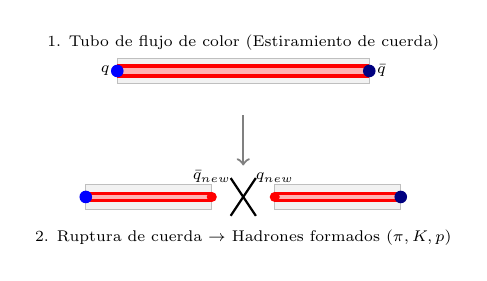
\begin{tikzpicture}[scale=0.8, transform shape]
                % Estado 1: Tubo de flujo estirándose (Línea doble gruesa)
                \draw[lightgray, fill=gray!10] (-2,1) rectangle (2,1.4);
                \draw[line width=1.5pt, double=red!30, double distance=2pt, red] (-2,1.2) -- (2,1.2);
                \fill[blue] (-2,1.2) circle (0.1);
                \node[left, black] at (-2,1.2) {\scriptsize $q$};
                \fill[blue!50!black] (2,1.2) circle (0.1);
                \node[right, black] at (2,1.2) {\scriptsize $\bar{q}$};
                \node[above] at (0,1.4) {\scriptsize 1. Tubo de flujo de color (Estiramiento de cuerda)};
                
                % Estado 2: Ruptura de cuerda
                \draw[lightgray, fill=gray!10] (-2.5,-1) rectangle (-0.5,-0.6);
                \draw[lightgray, fill=gray!10] (0.5,-1) rectangle (2.5,-0.6);
                \draw[line width=1.2pt, double=red!30, double distance=1.5pt, red] (-2.5,-0.8) -- (-0.5,-0.8);
                \draw[line width=1.2pt, double=red!30, double distance=1.5pt, red] (0.5,-0.8) -- (2.5,-0.8);
                
                % Ruptura (Snap)
                \draw[thick, black] (-0.2,-0.5) -- (0.2,-1.1);
                \draw[thick, black] (-0.2,-1.1) -- (0.2,-0.5);
                
                \fill[blue] (-2.5,-0.8) circle (0.1);
                \fill[red] (-0.5,-0.8) circle (0.08);
                \node[above] at (-0.5,-0.7) {\scriptsize $\bar{q}_{new}$};
                \fill[red] (0.5,-0.8) circle (0.08);
                \node[above] at (0.5,-0.7) {\scriptsize $q_{new}$};
                \fill[blue!50!black] (2.5,-0.8) circle (0.1);
                \node[below] at (0,-1.2) {\scriptsize 2. Ruptura de cuerda $\rightarrow$ Hadrones formados ($\pi, K, p$)};
                
                % Conexión dinámica
                \draw[->, thick, gray] (0,0.5) -- (0,-0.3);
            \end{tikzpicture}
\end{document}